
\documentclass[a4paper,12pt]{article}
\usepackage[a4paper,top=1.3cm,bottom=2cm,left=1.5cm,right=1.5cm,marginparwidth=0.75cm]{geometry}
\usepackage{cmap}					
\usepackage[warn]{mathtext} 		
\usepackage[T2A]{fontenc}			
\usepackage[utf8]{inputenc}			 
\usepackage[english,russian]{babel}	
\usepackage{longtable}
\usepackage{float}
\restylefloat{table}
\usepackage{graphicx}
\usepackage{tabularx}
\usepackage{hyperref}
\usepackage[rgb]{xcolor}
\usepackage{amsmath,amsfonts,amssymb,amsthm,mathtools} 
\mathtoolsset{showonlyrefs=true}
\usepackage{euscript}
\usepackage{mathrsfs}
\date{\today}
\begin{document}

\begin{titlepage}
	\begin{center}
		{\large МФТИ}
	\end{center}
	\begin{center}
		{\large ФРКТ}
	\end{center}
	
	
	\vspace{4.5cm}
	{\huge
		\begin{center}
			{\bf Лабораторная работа 5.1.2}\\
			Исследование эффекта Комптона.
		  
		

		\end{center}
	}
	\vspace{9cm}
	\begin{flushright}
		{\LARGE  $\newline$Добровольская Ксеня$\newline$Гаврилин Илья$\newline$
			\vspace{0.2cm}
			Б01-110$\newline$}
	\end{flushright}
	\vspace{8cm}
	
\end{titlepage}

\section{Аннотация}


   В данной работе предлагалось с помощью сцинтилляционного спектрометра исследовать энергетический спектр $\gamma$-квантов, рассеянных на графите. Определить энергию рассеянных $\gamma$-квантов в зависимости от угла рассеяния, а также энергию покоя частиц, на которых происходит комптоновское рассеяние. Ее значение составило $E = (523\pm 13)$кэВ, что отличается от табличного всего лишь на 2\% и совпадает с учетом погрешности.

  
\section{Теоретические сведения}

Рассеяние $\gamma$-лучей в веществе относится к числу явлений, в которых особенно ясно проявляется двойственная природа излучения. Волновая теория, хорошо объясняющая рассеяние длинноволнового излучения, испытывает трудности при описании рассеяния рентгеновских и $\gamma$-лучей. Эта теория, в частности, не может объяснить, почему в составе рассеянного излучения, измеренного Комптоном, кроме исходной волны с частотой $\omega_0$ появляется дополнительная длинноволновая компонента, отсутствующая в спектре первичного излучения.
	
	Появление этой компоненты легко объяснимо, если считать, что $\gamma$-излучение представляет собой поток квантов (фотонов), имеющих энергию $\hbar \omega$ и импульс $p = \hbar \omega / c$. Эффект Комптона — увеличение длины волны рассеянного излучения по сравнению с падающим -- интерпретируется как результат упругого соударения двух частиц: $\gamma$-кванта (фотона) и свободного электрона.
	
	Нетрудно получить, что изменение длины волны рассеянного излучения равно
	
	\[\Delta \lambda = \lambda_1 - \lambda_0 = \Lambda_\text{к} (1 - \cos\theta)\]
	
	, где $\lambda_0$ и $\lambda_1$ -- длины волн $\gamma$-кванта до и после рассеяния, а величина
	
	
	\[	\Lambda_\text{к} = \frac{h}{mc} = 2,42 \cdot 10^{-10} \text{ см}\]
	
	-- комптоновская длина волны электрона.
 
 
 	Кроме рассеяния $\gamma$-кванты испытывают в среде поглощение, вызываемое фотоэффектом и рождением электрон позитронных пар. Процесс рождения пар пороговый, он возможен лишь при энергии $\gamma$-квантов больше $2mc^2 = 1,02$ МэВ и в рассматриваемом энергетическом диапазоне не происходит. При фотоэффекте из атома выбивается электрон, а квант поглощается. Импульс кванта делится между вылетевшим электроном и атомом, а его энергия частично передается электрону, а частично тратится на возбуждение атома. Атом практически мгновенно (за время порядка $10^{-8}$ с) возвращается в нормальное состояние. Его энергия возбуждения либо излучается в виде мягкого фотона, либо передается какому-нибудь другому электрону, который покидает атом (Оже-эффект). И в том, и в другом случае энергия возбуждения обычно поглощается соседними атомами рассеивателя. Основной целью данной работы является проверка соотношения для $\Delta \lambda $. Применительно к условиям нашего опыта эту формулу следует преобразовать от длин волн к энергии $\gamma$-квантов. Как нетрудно показать, соответствующее выражение имеет вид
 
 \[\frac{1}{\varepsilon(\theta)} - \frac{1}{\varepsilon(0)} = 1 - \cos\theta\]
 
 	, где $\varepsilon(0) = \dfrac{E_0}{mc^2}$ -- выраженная в единицах $mc^2$ энергия $\gamma$-квантов, падающих на рассеиватель, $\varepsilon(\theta)$ -- выраженная в тех же единицах энергия квантов, испытавших комптоновское рассеяние на угол $\theta$, а $m$ -- масса электрона.
	
	Заменим в формуле энергию квантов, испытавших комптоновское рассеяние на угол $\theta$, номером канала $N(\theta)$, соответствующего вершине фотопика при указанном угле $\theta$. Обозначая буквой $A$ неизвестный коэффициент пропорциональности между $\varepsilon(\theta)$ и $N(\theta)$, найдем:
	
	\[	\frac{1}{N(\theta)} - \frac{1}{N(0)} = A(1 - \cos\theta)\]
	
		\[	\frac{1}{N(\theta)} = \frac{1}{N(0)} + A(1 - \cos\theta)\]
	
	
	Возвращаясь от переменной $\varepsilon$ к энергии $E$, мы получаем, что при $\theta = 90^\circ$ формула принимает вид

\[mc^2 \left(\frac{1}{E(90)} - \frac{1}{E(0)}\right) = 1\]

 или

\[		mc^2 = E(0)\frac{E(90)}{E(0) - E(90)} = E_\gamma \frac{N(90)}{N(0) - N(90)}\]
	
	В этой формуле $E(0) = E_\gamma$ -- энергия электронов, рассеянных вперед, -- просто равна энергии $\gamma$-лучей, испускаемых источником.
	
	
	
\section{Экспериментальная установка} 
   
   
Схема экспериментальной установки приведена на рис.1.
  
    \begin{figure}[H]
  \begin{center}
    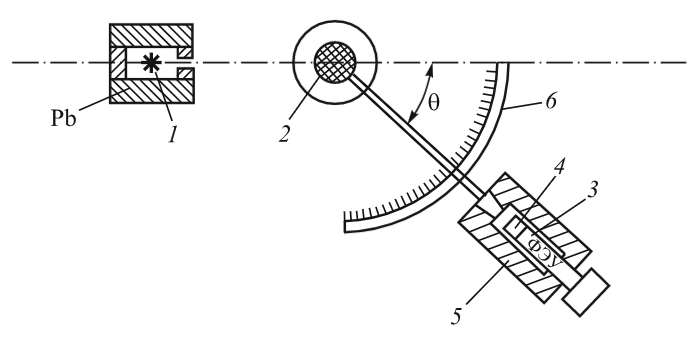
\includegraphics[width=10cm]{ex1.png}
    \caption{Схема экспериментальной установки.}
    \label{fig:}
  \end{center}
\end{figure}
 
Источником излучения 1 служит $^{137}$Cs, испускающий $\gamma$-лучи с энергией 662 кэВ. Он помещен в толстостенный свинцовый контейнер с коллиматором. Сформированный коллиматором узкий пучок $\gamma$-квантов попадает на графитовую мишень 2 (цилиндр диаметром 40 мм и высотой 100 мм).
 
 	Кванты, испытавшие комптоновское рассеяние в мишени, регистрируются сцинтилляционным счетчиком. Счетчик состоит из фотоэлектронного умножителя 3 (далее ФЭУ) и сцинтиллятора 4. Сцинтиллятором служит
 	кристалл NaI(Tl) цилиндрической формы диаметром 40 мм и высотой 40 мм, его выходное окно находится в оптическом контакте с фотокатодом ФЭУ. Сигналы, возникающие на аноде ФЭУ, подаются на ЭВМ для амплитудного анализа. Кристалл и ФЭУ расположены в светонепроницаемом блоке, укрепленном на горизонтальной штанге. Штанга вместе с этим блоком может вращаться относительно мишени, угол поворота отсчитывается по лимбу 6.
 	
 	Головная часть сцинтилляционного блока закрыта свинцовым коллиматором 5, который формирует входной пучок и защищает детектор от постороннего излучения. Основной вклад в это излучение вносят $\gamma$-кванты, проходящие из источника 1 через 6-сантиметровые стенки защитного контейнера. Этот фон особенно заметен при исследовании комптоновского рассеяния на большие углы ($\simeq 120^\circ$), когда расстояние между детектором и источником уменьшается.
 	
 	
 	Под действием монохроматического излучения на выходе ФЭУ возникает распределение электрических импульсов. В амплитудном распределении импульсов имеется так называемый фотопик, возникающий в результате фотоэффекта, и обязанное комптоновскому рассеянию сплошное распределение. Часто фотопик называется также пиком полного поглощения, его положение однозначно связана с энергией регистрируемого $\gamma$-излучения.Нас будет интересовать положение (номер канала) вершины этого пика в зависимости от угла поворота детектора.
	
	
\section{Измерения и обработка результатов} 
 
 \begin{enumerate}
		\item Включим все измерительные устройства и компьютер.
		
		\item Запустим программу и войдем в режим измерения спектра.
		
		    \begin{figure}[H]
  \begin{center}
    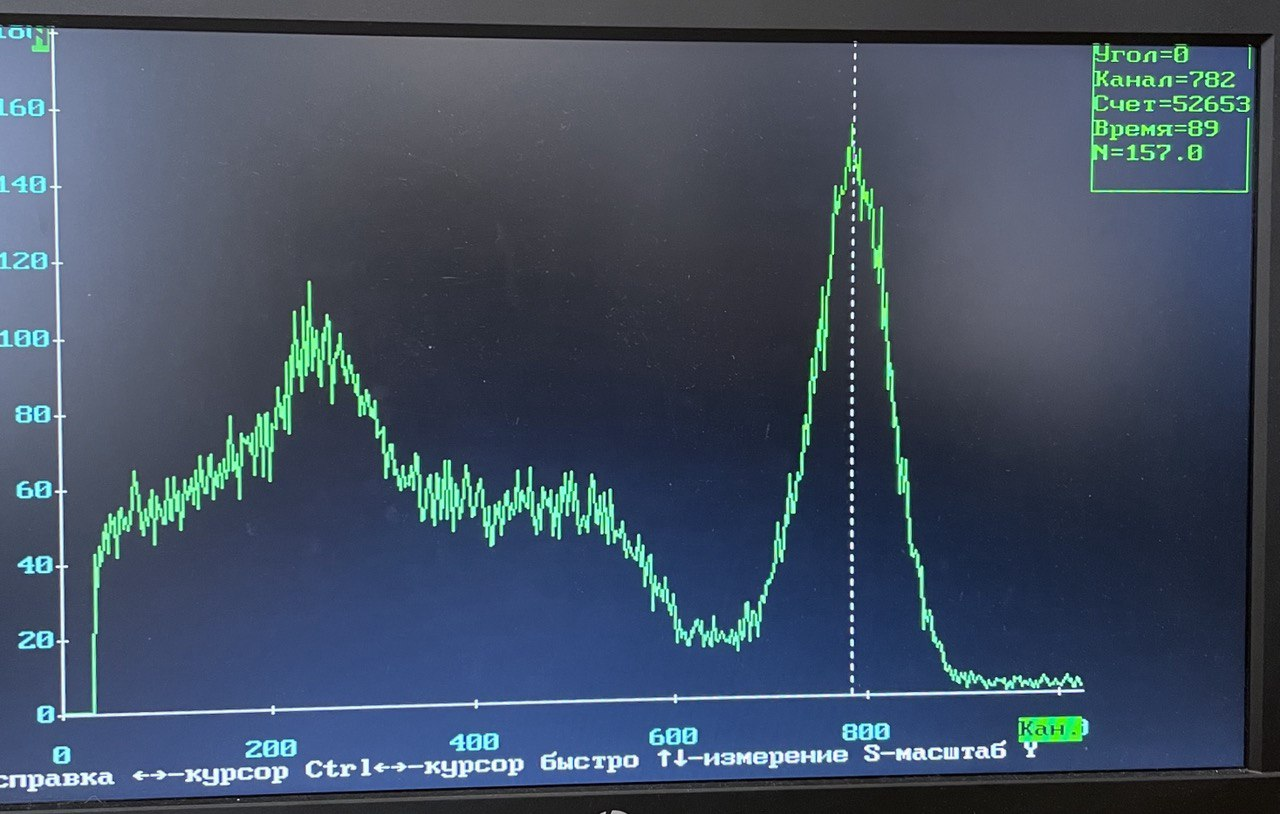
\includegraphics[width=12cm]{ex2.jpg}
    \caption{Амплитудные спектры.}
    \label{fig:}
  \end{center}
\end{figure}

		\item Устанавливая сцинтилляционный счетчик под разными углами $\theta$ к первоначальному направлению полета $\gamma$-квантов и вводя значения этих углов в ЭВМ, снимем амплитудные спектры и определим положения фотопиков для каждого значения угла $\theta$; измерения проведем с шагом $10^\circ$ в диапазоне от $0^\circ$ до $120^\circ$. Результаты запишем в таблицу:
		
  \begin{table}[H]
\begin{center}
\begin{tabular}{|c|c|c|c|c|c|c|c|c|c|c|c|c|c|}
\hline $\theta, \circ$&0&10&20&30&40&50&60&70&80&90&100&110&120\\
\hline $N ,$шт&783&779&681&651&580&505&457&412&360&328&304&282&264\\
\hline $\Delta_N, $ шт&8&8&7&7&6&5&5&4&4&3&3&3&3\\
\hline
\end{tabular}
\end{center}
\end{table}

, где абсолютная погрешность измерения по счетчику
\[ \Delta_N = \sqrt{(\Delta_N)_{\text{приб}}^2 + (\Delta_N)_{\text{изм}}^2} \]


$(\Delta_N)_{\text{приб}} = 0.01N, (\Delta_N)_{\text{изм}} = 1$

\item 	Используя экспериментальные результаты, построим график, откладывая по оси абсцисс величину $1 - \cos\theta$, по оси ординат --- $1 / N(\theta)$ и ее ошибку. Проведем через полученные точки наилучшую прямую:

	\[	\frac{1}{N(\theta)} = \frac{1}{N(0)} + A(1 - \cos\theta) = k (1 - \cos\theta) + b\]
	

		    \begin{figure}[H]
  \begin{center}
    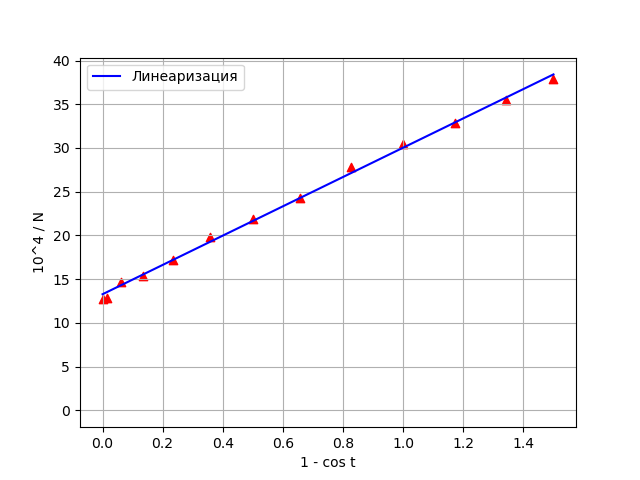
\includegraphics[width=15cm]{gra1.png}
    \caption{График зависимости $10^4$ / N от $(1 - \cos\theta)$.}
    \label{fig:}
  \end{center}
\end{figure}

\item Коэффициенты определяем из графика:

k = $(16,8\pm0.2) * 10^4$


b = $(13,28\pm0.13) * 10^4$


\item Определив коэффициенты в графике, найдем энергию покоя частицы, на которой происходит комптоновское рассеяние первичных $\gamma$-квантов, $E_\gamma = 662$кэВ:

\[E = mc^2 = E(0)\frac{E(90)}{E(0) - E(90)} = E_\gamma \frac{N(90)}{N(0) - N(90)}\]

, где 
\[ \frac{1}{N(0)} = b => N(0) = \frac{1}{b} = (7.53 \pm 0.08)* 10^6\]
\[ \frac{1}{N(90)} = k + b => N(90) = \frac{1}{k + b} = (3.32 \pm 0.03)* 10^6\]

\[E = mc^2 = (0.79 \pm 0.02) E_\gamma = (523 \pm 13)keB\]
		
\item Табличное значение покоя электрона - $E_e = 511 keB$. Таким образом, отклонение от табличного значения - 2\%.
	\end{enumerate}



\section{Выводы}

В данной работе мы исследовали эффект Комптона. Наблюдали энергетический спектр рассеянных $\gamma$-квантов в зависимости от угла рассеяния. Также определили энергию покоя частиц, на которых происходит рассеяние, ее значение составило  $E = (523\pm 13)$кэВ, что подтверждает рассеяние именно на электронах. Табличное значение энергии покоя электрона - 511 кЭв, то есть измеренное значение отличается от табличного всего лишь на 2 \% и совпадает с учетом погрешности, что говорит о хорошей точности измерений и применимости данного метода.

\end{document}
	
